\documentclass{article}%
\usepackage[T1]{fontenc}%
\usepackage[utf8]{inputenc}%
\usepackage{lmodern}%
\usepackage{textcomp}%
\usepackage{lastpage}%
\usepackage{parskip}%
\usepackage[top=1.2in,bottom=1in,left=0.6in,right=0.6in,headsep=0.8in]{geometry}%
\usepackage{amsmath}%
\usepackage{graphicx}%
\usepackage{needspace}%
\usepackage{color}%
\usepackage{longtable}%
\usepackage{multirow}%
\usepackage[table]{xcolor}%
\usepackage{fancyhdr}%
\usepackage{tabularx}%
%
\definecolor{OsdagGreen}{HTML}{D5DF93}%
\fancypagestyle{header}{ 
\renewcommand{\headrulewidth}{0pt}%
\renewcommand{\footrulewidth}{0pt}%
\fancyhead{ 
}%
\fancyfoot{ 
}%
\fancyhead[C]{ 
\begin{tabularx}{\textwidth}{|l|p{6cm}|l|X|}%
\hline%
\rowcolor{OsdagGreen}%
Company Name&&Project Title&\\%
\hline%
\rowcolor{OsdagGreen}%
Group/Team Name&&Subtitle&\\%
\hline%
\rowcolor{OsdagGreen}%
Designer&&Job Number&\\%
\hline%
\rowcolor{OsdagGreen}%
Date&11 /05 /2020&Client&\\%
\hline%
\end{tabularx}
}%
\fancyfoot[R]{ 
Page \thepage\ of \pageref{LastPage}
}
}%
%
\begin{document}%
\normalsize%
\pagestyle{header}%
\section{Input Parameters}%
\label{sec:InputParameters}%
\renewcommand{\arraystretch}{1.2}%
\begin{longtable}{|p{5cm}|p{2cm}|p{2cm}|p{2cm}|p{5cm}|}%
\hline%
\hline%
\multicolumn{3}{|c|}{Module}&\multicolumn{2}{|c|}{Beam Coverplate Connection}\\%
\hline%
\hline%
\multicolumn{3}{|c|}{MainModule}&\multicolumn{2}{|c|}{Moment Connection}\\%
\hline%
\hline%
\multicolumn{3}{|c|}{Moment(kNm)*}&\multicolumn{2}{|c|}{10.0}\\%
\hline%
\hline%
\multicolumn{3}{|c|}{Shear(kN)*}&\multicolumn{2}{|c|}{10.0}\\%
\hline%
\hline%
\multicolumn{3}{|c|}{Axial (kN) *}&\multicolumn{2}{|c|}{10.0}\\%
\hline%
\hline%
\multicolumn{5}{|c|}{\textbf{Section}}\\%
\hline%
\hline%
\multirow{13}{*}{\includegraphics[width=5cm,height=5cm]{C:/Users/Priti/Desktop/Osdag3/ResourceFiles/images/ISection".png}}&\multicolumn{2}{|c|}{Beam Section *}&\multicolumn{2}{|c|}{NPB 330x160x49.1}\\%
\cline{2%
-%
5}%
&\multicolumn{2}{|c|}{Preferences}&\multicolumn{2}{|c|}{Outside}\\%
\cline{2%
-%
5}%
&\multicolumn{2}{|c|}{Material *}&\multicolumn{2}{|c|}{E 250 (Fe 410 W)A}\\%
\cline{2%
-%
5}%
&\multicolumn{2}{|c|}{Ultimate strength, fu (MPa)}&\multicolumn{2}{|c|}{410}\\%
\cline{2%
-%
5}%
&Yield Strength , fy (MPa)&230&R2(mm)&0.0\\%
\cline{2%
-%
5}%
&Mass&49.15&Iz(mm4)&117669000.0\\%
\cline{2%
-%
5}%
&Area(mm2) {-} A&6260.0&Iy(mm4)&7869000.0\\%
\cline{2%
-%
5}%
&D(mm)&330.0&rz(mm)&137.10000000000002\\%
\cline{2%
-%
5}%
&B(mm)&160.0&ry(mm)&35.5\\%
\cline{2%
-%
5}%
&t(mm)&7.5&Zz(mm3)&713150.0\\%
\cline{2%
-%
5}%
&T(mm)&11.5&Zy(mm3)&98360.0\\%
\cline{2%
-%
5}%
&FlangeSlope&90&Zpz(mm3)&804330.0\\%
\cline{2%
-%
5}%
&R1(mm)&1.8&Zpy(mm3)&98360.0\\%
\cline{2%
-%
5}%
\hline%
\multicolumn{5}{|c|}{\textbf{Bolt Details}}\\%
\hline%
\hline%
\multicolumn{3}{|c|}{Diameter (mm)*}&\multicolumn{2}{|c|}{{[}12.0, 16.0, 20.0, 24.0, 30.0, 36.0{]}}\\%
\hline%
\hline%
\multicolumn{3}{|c|}{Grade *}&\multicolumn{2}{|c|}{{[}3.6, 4.6, 4.8, 5.6, 5.8, 6.8, 8.8, 9.8, 10.9, 12.9{]}}\\%
\hline%
\hline%
\multicolumn{3}{|c|}{Type *}&\multicolumn{2}{|c|}{Bearing Bolt}\\%
\hline%
\hline%
\multicolumn{3}{|c|}{Bolt.fu}&\multicolumn{2}{|c|}{500.0}\\%
\hline%
\hline%
\multicolumn{3}{|c|}{Bolt.fy}&\multicolumn{2}{|c|}{300.0}\\%
\hline%
\hline%
\multicolumn{3}{|c|}{Bolt hole type}&\multicolumn{2}{|c|}{Standard}\\%
\hline%
\hline%
\multicolumn{3}{|c|}{Slip factor (µ\_f)}&\multicolumn{2}{|c|}{0.3}\\%
\hline%
\hline%
\multicolumn{3}{|c|}{Type of edges}&\multicolumn{2}{|c|}{a {-} Sheared or hand flame cut}\\%
\hline%
\hline%
\multicolumn{3}{|c|}{Gap between beam and <br>support (mm)}&\multicolumn{2}{|c|}{10.0}\\%
\hline%
\hline%
\multicolumn{3}{|c|}{Are the members exposed to <br>corrosive influences}&\multicolumn{2}{|c|}{False}\\%
\hline%
\end{longtable}

%
\Needspace{10\baselineskip}%
\newpage%
\section{Design Checks}%
\label{sec:DesignChecks}%
\subsection{Member Capacity}%
\label{subsec:MemberCapacity}%
\renewcommand{\arraystretch}{1.2}%
\begin{longtable}{|p{4cm}|p{5cm}|p{5.5cm}|p{1.5cm}|}%
\hline%
\rowcolor{OsdagGreen}%
Check&Required&Provided&Remarks\\%
\hline%
\endhead%
\hline%
Axial Capacity (kN)&&$\begin{aligned} Ac &=\frac{A*f_y}{\gamma_{m0} *1000}\\ &=\frac{6260.0*230}{1.1* 1000}\\ &=1308.91\end{aligned}$&\\%
\hline%
Shear Capacity (kN)&&$\begin{aligned} S_c &= \frac{A_v*f_y}{\sqrt{3}*\gamma_{mo} *1000}\\ &=\frac{307.0*7.5*230}{\sqrt{3}*1.1 *1000}\\ &=277.95\end{aligned}$&\\%
\hline%
Plastic Moment Capacity (kNm)&&$\begin{aligned} Pmc &= \frac{\beta_b * Z_p *fy}{\gamma_{mo} * 1000000}\\ &=\frac{1*176717*230}{1.1 * 1000000}\\ &=36.95\end{aligned}$&\\%
\hline%
Moment Deformation Criteria (kNm)&&$\begin{aligned} Mdc &= \frac{1.5 *Z_e *fy}{1.1 * 1000000}\\ &= \frac{1.5 *713150.0*230}{1.1 * 1000000}\\ &= 223.67\end{aligned}$&\\%
\hline%
Moment Capacity (kNm)&&$\begin{aligned} M_c &= min(Pmc,Mdc)\\ &=min(36.95,223.67)\\ &=36.95\end{aligned}$&\\%
\hline%
\end{longtable}

%
\newpage%
\subsection{Load Considered}%
\label{subsec:LoadConsidered}%
\renewcommand{\arraystretch}{1.2}%
\begin{longtable}{|p{4cm}|p{5cm}|p{5.5cm}|p{1.5cm}|}%
\hline%
\rowcolor{OsdagGreen}%
Check&Required&Provided&Remarks\\%
\hline%
\endhead%
\hline%
Axial Load (kN)&$\begin{aligned} Ac_{min} &= 0.3 * A_c\\ &= 0.3 *1308.91\\ &=392.67\end{aligned}$&$\begin{aligned} Au &= max(A,Ac_{min} )\\ &= max( 10.0,392.67)\\ &=392.67\end{aligned}$&Pass\\%
\hline%
Shear Load (kN)&$\begin{aligned} Vc_{min} &= 0.6 * S_c\\ &= 0.6 *277.95\\ &=166.77\end{aligned}$&$\begin{aligned} Vu &= max(V,Vc_{min})\\ &=  max(10.0,166.77)\\ &=166.77\end{aligned}$&Pass\\%
\hline%
Moment Load (kNm)&$\begin{aligned} Mc_{min} &= 0.5 * M_c\\ &= 0.5 *36.95\\ &=18.47\end{aligned}$&$\begin{aligned} Mu &= max(M,Mc_{min} )\\ &= max(10.0,18.47)\\ &=18.47\end{aligned}$&Pass\\%
\hline%
Forces Carried by Web&&$\begin{aligned}A_w &= Axial~ force~ in~ web  \\   &= \frac{(D- 2*T)*t* Au }{A} \\ &= \frac{(330.0- 2*11.5)*7.5*392.67 }{6260.0} \\ &=144.43\\ M_w &= Moment ~in ~web  \\  &= \frac{Z_w * Mu}{Z} \\ &= \frac{176717 * 18.47}{804330.0} \\ &=4.06\end{aligned}$&\\%
\hline%
Forces Carried by Flange&&$\begin{aligned} A_f&= Axial~force~ in ~flange  \\ &= \frac{Au * B *T}{A} \\ &= \frac{392.67 * 160.0*11.5}{6260.0} \\ &=115.42\\ M_f& =Moment~ in~ flange \\  & = Mu-M_w\\ &= 18.47-4.06\\ &=14.42\\  F_f& =flange~force  \\ & = \frac{M_f *1000}{D-T} + A_f \\ &= \frac{14.42*1000}{330.0-11.5} +115.42 \\ &=160.68\end{aligned}$&\\%
\hline%
\end{longtable}

%
\newpage%
\subsection{Flange Bolt Checks}%
\label{subsec:FlangeBoltChecks}%
\renewcommand{\arraystretch}{1.2}%
\begin{longtable}{|p{4cm}|p{5cm}|p{5.5cm}|p{1.5cm}|}%
\hline%
\rowcolor{OsdagGreen}%
Check&Required&Provided&Remarks\\%
\hline%
\endhead%
\hline%
Diameter (mm)&Bolt Quantity Optimisation&$\begin{aligned} d &=12.0 \end{aligned}$&\\%
\hline%
Grade&Bolt Grade Optimisation&5.6&\\%
\hline%
Hole Diameter (mm)& &$\begin{aligned} d_0 &=13.0 \end{aligned}$&\\%
\hline%
Shear Capacity (kN)&&$\begin{aligned}V_{dsb} &= \frac{f_{ub} ~n_n~ A_{nb}}{1000*\sqrt{3} ~\gamma_{mb}}\\ &= \frac{500.0*1*84.3}{1000*\sqrt{3}~*~1.25}\\ &= 19.47\end{aligned}$&\\%
\hline%
Bearing Capacity (kN)&&$\begin{aligned}V_{dpb} &= \frac{2.5~ k_b~ d~ t~ f_u}{1000*\gamma_{mb}}\\ &= \frac{2.5~*0.52*12.0*11.5*410}{1000*1.25}\\ &=58.84\end{aligned}$&\\%
\hline%
Bolt Capacity (kN)&&$\begin{aligned}V_{db} &= min~ (V_{dsb}, V_{dpb})\\ &= min~ (19.47,58.84)\\ &=19.47\end{aligned}$&\\%
\hline%
No of Bolts&$\begin{aligned}R_{u} &= \sqrt{V_u^2+A_u^2}\\ n_{trial} &= R_u/ V_{bolt}\\ R_{u} &= \frac{\sqrt{0.0^2+160.68^2}}{19.47}\\ &=18\end{aligned}$&20&\\%
\hline%
No of Columns&&$\begin{aligned} n_c &=10 \end{aligned}$&\\%
\hline%
No of Rows&&$\begin{aligned} n_r &=2 \end{aligned}$&\\%
\hline%
Min. Pitch (mm)&$\begin{aligned}p/g_{min}&= 2.5 ~ d&\\ =&2.5*12.0&=30.0\end{aligned}$&30&Pass\\%
\hline%
Max. Pitch (mm)&$\begin{aligned}p/g_{max} &=\min(32~t,~300~mm)&\\ &=\min(32 *~11.5,~ 300 ~mm)\\&=300\end{aligned}$&30&Pass\\%
\hline%
Min. Gauge (mm)&$\begin{aligned}p/g_{min}&= 2.5 ~ d&\\ =&2.5*12.0&=30.0\end{aligned}$&0.0&N/A\\%
\hline%
Max. Gauge (mm)&$\begin{aligned}p/g_{max} &=\min(32~t,~300~mm)&\\ &=\min(32 *~11.5,~ 300 ~mm)\\&=300\end{aligned}$&0.0&N/A\\%
\hline%
Min. End Distance (mm)&$\begin{aligned}e/e`_{min} &=[1.5~or~ 1.7] * d_0\\ &=1.7*13.0=22.1 \end{aligned}$&25&Pass\\%
\hline%
Max. End Distance (mm)&$\begin{aligned}e/e`_{max} &= 12~ t~ \varepsilon&\\ \varepsilon &= \sqrt{\frac{250}{f_y}}\\ e/e`_{max}&=12 ~*14.0*\sqrt{\frac{250}{230}}\\ &=174.72\\ \end{aligned}$&25&Pass\\%
\hline%
Min. Edge Distance (mm)&$\begin{aligned}e/e`_{min} &=[1.5~or~ 1.7] * d_0\\ &=1.7*13.0=22.1 \end{aligned}$&37.225&Pass\\%
\hline%
Max. Edge Distance (mm)&$\begin{aligned}e/e`_{max} &= 12~ t~ \varepsilon&\\ \varepsilon &= \sqrt{\frac{250}{f_y}}\\ e/e`_{max}&=12 ~*14.0*\sqrt{\frac{250}{230}}\\ &=174.72\\ \end{aligned}$&37.225&Pass\\%
\hline%
Long Joint Reduction&$\begin{aligned} &if~l\geq 15 * d~then~V_{rd} = \beta_{ij} * V_{db} \\ & if~l < 15 * d~then~V_{rd} = V_{db} \\ & where,\\ & l = ((nc~or~nr) - 1) * (p~or~g) \\ & \beta_{ij} = 1.075 - l/(200 * d) \\ & but~0.75\leq\beta_{ij}\leq1.0 \end{aligned}$&$\begin{aligned} l&= ((nc~or~nr) - 1) * (p~or~g) \\  &= (10 - 1) * 30=270\\  &= (2 - 1) * 0.0=0.0\\  l&= 270\\ & 15 * d = 15 * 12.0 = 180.0 \\ & since,~l \geq 15 * d~then~V_{rd} = \beta_{ij} * V_{db} \\ & \beta_{ij} = 1.075 - 270/(200*12.0) =0.96\\ & V_{rd} = 0.96 * 19.47=19468.25 \end{aligned}$&\\%
\hline%
\end{longtable}

%
\newpage%
\subsection{Web Bolt Checks}%
\label{subsec:WebBoltChecks}%
\renewcommand{\arraystretch}{1.2}%
\begin{longtable}{|p{4cm}|p{5cm}|p{6.5cm}|p{1.5cm}|}%
\hline%
\rowcolor{OsdagGreen}%
Check&Required&Provided&Remarks\\%
\hline%
\endhead%
\hline%
Shear Capacity (kN)&&$\begin{aligned}V_{dsb} &= \frac{f_{ub} ~n_n~ A_{nb}}{1000*\sqrt{3} ~\gamma_{mb}}\\ &= \frac{500.0*2*84.3}{1000*\sqrt{3}~*~1.25}\\ &= 38.94\end{aligned}$&\\%
\hline%
Bearing Capacity (kN)&&$\begin{aligned}V_{dpb} &= \frac{2.5~ k_b~ d~ t~ f_u}{1000*\gamma_{mb}}\\ &= \frac{2.5~*0.52*12.0*7.5*410}{1000*1.25}\\ &=38.38\end{aligned}$&\\%
\hline%
Bolt Capacity (kN)&&$\begin{aligned}V_{db} &= min~ (V_{dsb}, V_{dpb})\\ &= min~ (38.94,38.38)\\ &=38.38\end{aligned}$&\\%
\hline%
No of Bolts&$\begin{aligned}R_{u} &= \sqrt{V_u^2+A_u^2}\\ n_{trial} &= R_u/ V_{bolt}\\ R_{u} &= \frac{\sqrt{166.77^2+144.43^2}}{38.38}\\ &=12\end{aligned}$&20&\\%
\hline%
No of Columns&&$\begin{aligned} n_c &=4 \end{aligned}$&\\%
\hline%
No of Rows&&$\begin{aligned} n_r &=5 \end{aligned}$&\\%
\hline%
Min. Pitch (mm)&$\begin{aligned}p/g_{min}&= 2.5 ~ d&\\ =&2.5*12.0&=30.0\end{aligned}$&30&Pass\\%
\hline%
Max. Pitch (mm)&$\begin{aligned}p/g_{max} &=\min(32~t,~300~mm)&\\ &=\min(32 *~6.0,~ 300 ~mm)\\&=192.0\end{aligned}$&30&Pass\\%
\hline%
Min. Gauge (mm)&$\begin{aligned}p/g_{min}&= 2.5 ~ d&\\ =&2.5*12.0&=30.0\end{aligned}$&65&Pass\\%
\hline%
Max. Gauge (mm)&$\begin{aligned}p/g_{max} &=\min(32~t,~300~mm)&\\ &=\min(32 *~6.0,~ 300 ~mm)\\&=192.0\end{aligned}$&65&Pass\\%
\hline%
Min. End Distance (mm)&$\begin{aligned}e/e`_{min} &=[1.5~or~ 1.7] * d_0\\ &=1.7*13.0=22.1 \end{aligned}$&25&Pass\\%
\hline%
Max. End Distance (mm)&$\begin{aligned}e/e`_{max} &= 12~ t~ \varepsilon&\\ \varepsilon &= \sqrt{\frac{250}{f_y}}\\ e/e`_{max}&=12 ~*6.0*\sqrt{\frac{250}{230}}\\ &=74.88\\ \end{aligned}$&25&Pass\\%
\hline%
Min. Edge Distance (mm)&$\begin{aligned}e/e`_{min} &=[1.5~or~ 1.7] * d_0\\ &=1.7*13.0=22.1 \end{aligned}$&25&Pass\\%
\hline%
Max. Edge Distance (mm)&$\begin{aligned}e/e`_{max} &= 12~ t~ \varepsilon&\\ \varepsilon &= \sqrt{\frac{250}{f_y}}\\ e/e`_{max}&=12 ~*6.0*\sqrt{\frac{250}{230}}\\ &=74.88\\ \end{aligned}$&25&Pass\\%
\hline%
Parameters required for bolt force&&$\begin{aligned} l_n~~~ &= length~available \\  l_n~~~ &= (n_r - 1) * g\\  &= (5 - 1) *65\\  & =260\\  y_{max} &= l_n / 2\\  &= 260 / 2 \\  & =130.0\\ x_{max} &= p * (n_c - 1) / 2 \\  &= 30 * (4 - 1) / 2 \  & =15.0\end{aligned}$&\\%
\hline%
Moment Demand&&$\begin{aligned}  M_d~~ &= (V_u * ecc + M_w)\\  &= (166.77 * 45.0 + 4.06)\\  & =11.56\end{aligned}$&\\%
\hline%
Bolt.Force&&$\begin{aligned} vbv~~ &= V_u / (n_r * n_c)\\  &= \frac{166.77}{ (5*4)}\\  & =16.68\\ tmh~ &= \frac{M_d * y_{max} }{ \Sigma r_i^2} \\  &= \frac{11.56 *130.0}{86.75}\\  & =17.33\\  tmv ~&= \frac{M_d * x_{max}}{\Sigma r_i^2}\\ &= \frac{11.56 * 15.0}{86.75}\\  & =2.0\\  abh~ & = \frac{A_u }{(n_r * n_c)}\\   & =\frac{144.43}{ (5 *4)}\\  & =14.44\\  vres &=\sqrt{(vbv +tmv) ^ 2 + (tmh+abh) ^ 2}\\   &= \sqrt{(16.68 +2.0) ^2 + (17.33+14.44) ^ 2}\\  & =36.85\end{aligned}$&\\%
\hline%
Long Joint Reduction&$\begin{aligned} &if~l\geq 15 * d~then~V_{rd} = \beta_{ij} * V_{db} \\ & if~l < 15 * d~then~V_{rd} = V_{db} \\ & where,\\ & l = ((nc~or~nr) - 1) * (p~or~g) \\ & \beta_{ij} = 1.075 - l/(200 * d) \\ & but~0.75\leq\beta_{ij}\leq1.0 \end{aligned}$&$\begin{aligned} l&= ((nc~or~nr) - 1) * (p~or~g) \\  &= (4 - 1) * 30=90\\  &= (5 - 1) * 65=260\\  l&= 260\\ & 15 * d = 15 * 12.0 = 180.0 \\ & since,~l \geq 15 * d~then~V_{rd} = \beta_{ij} * V_{db} \\ & \beta_{ij} = 1.075 - 260/(200*12.0) =0.97\\ & V_{rd} = 0.97 * 38.38=37.1 \end{aligned}$&\\%
\hline%
Capacity (kN)&36.85&37.1&Pass\\%
\hline%
\end{longtable}

%
\newpage%
\subsection{Outer flange plate Checks}%
\label{subsec:OuterflangeplateChecks}%
\renewcommand{\arraystretch}{1.2}%
\begin{longtable}{|p{4cm}|p{6cm}|p{5.5cm}|p{1.5cm}|}%
\hline%
\rowcolor{OsdagGreen}%
Check&Required&Provided&Remarks\\%
\hline%
\endhead%
\hline%
Min. Plate Height (mm)&$\begin{aligned}min~flange~plate~ht &= beam~width\\ &=160.0\end{aligned}$&160.0&Pass\\%
\hline%
Min. Plate Length (mm)&$\begin{aligned} & 2[2*e_{min} + ({\frac{bolt~lines}{2}}-1) * p_{min})]\\ & +\frac{gap}{2}]\\ &=2*[(2*22.1 + (\frac{10}{2}-1) * 30.0\\ &= + \frac{10.0}{2}]\\ &=338.4\end{aligned}$&350.0&Pass\\%
\hline%
Min.Plate Thickness (mm)&$\begin{aligned} t_w=11.5\end{aligned}$&14.0&Pass\\%
\hline%
\end{longtable}

%
\newpage%
\subsection{Member Checks}%
\label{subsec:MemberChecks}%
\renewcommand{\arraystretch}{1.2}%
\begin{longtable}{|p{4cm}|p{6cm}|p{5.5cm}|p{1.5cm}|}%
\hline%
\rowcolor{OsdagGreen}%
Check&Required&Provided&Remarks\\%
\hline%
\endhead%
\hline%
Flange Tension Yielding Capacity (kN)&&$\begin{aligned} T_{dg} &= \frac{l*t_p*f_y}{1000*\gamma_{mo}}\\ &=\frac{160.0*11.5*230}{1000*1.1}\\ &=384.73\end{aligned}$&\\%
\hline%
Flange Tension Rupture Capacity (kN)&&$\begin{aligned} T_{dn} &= \frac{0.9*A_{n}*f_u}{1000*\gamma_{m1}}\\ &=\frac{0.9*(160.0-2*13.0)*11.5*410}{1000*1.25}\\ &=454.9\end{aligned}$&\\%
\hline%
Flange Block Shear Capacity (kN)&&$\begin{aligned}T_{db1} &= \frac{A_{vg} f_{y}}{1000*\sqrt{3} \gamma_{m0}} + \frac{0.9 A_{tn} f_{u}}{1000*\gamma_{m1}}\\ T_{db2} &= \frac{0.9*A_{vn} f_{u}}{1000*\sqrt{3} \gamma_{m1}} + \frac{A_{tg} f_{y}}{1000*\gamma_{m0}}\\ T_{db} &= min(T_{db1}, T_{db2})= 518.1\end{aligned}$&\\%
\hline%
Flange Tension Capacity (kN)&$\begin{aligned} f_f &=160.68 \end{aligned}$&$\begin{aligned} T_d &= Min(T_{dg},T_{dn},T_{db})\\ &= Min(384.73,454.9,518.1)\\ &=384.73\end{aligned}$&Pass\\%
\hline%
Web Tension Yielding Capacity (kN)&&$\begin{aligned} T_{dg} &= \frac{l*t_p*f_y}{1000*\gamma_{mo}}\\ &=\frac{307.0*7.5*230}{1000*1.1}\\ &=481.43\end{aligned}$&\\%
\hline%
Web Tension Rupture Capacity (kN)&&$\begin{aligned} T_{dn} &= \frac{0.9*A_{n}*f_u}{1000*\gamma_{m1}}\\ &=\frac{0.9*(307.0-5*13.0)*7.5*410}{1000*1.25}\\ &=535.79\end{aligned}$&\\%
\hline%
Web Block Shear Capacity (kN)&&$\begin{aligned}T_{db1} &= \frac{A_{vg} f_{y}}{1000*\sqrt{3} \gamma_{m0}} + \frac{0.9 A_{tn} f_{u}}{1000*\gamma_{m1}}\\ T_{db2} &= \frac{0.9*A_{vn} f_{u}}{1000*\sqrt{3} \gamma_{m1}} + \frac{A_{tg} f_{y}}{1000*\gamma_{m0}}\\ T_{db} &= min(T_{db1}, T_{db2})= 615.45\end{aligned}$&\\%
\hline%
Web Tension Capacity (kN)&$\begin{aligned} A_w &=144.43 \end{aligned}$&$\begin{aligned} T_d &= Min(T_{dg},T_{dn},T_{db})\\ &= Min(481.43,535.79,615.45)\\ &=481.43\end{aligned}$&Pass\\%
\hline%
\end{longtable}

%
\newpage%
\subsection{Flange Plate Capacity Checks in Axial{-}Outside }%
\label{subsec:FlangePlateCapacityChecksinAxial{-}Outside}%
\renewcommand{\arraystretch}{1.2}%
\begin{longtable}{|p{4cm}|p{6cm}|p{5.5cm}|p{1.5cm}|}%
\hline%
\rowcolor{OsdagGreen}%
Check&Required&Provided&Remarks\\%
\hline%
\endhead%
\hline%
Tension Yielding Capacity (kN)&&$\begin{aligned} T_{dg} &= \frac{l*t_p*f_y}{1000*\gamma_{mo}}\\ &=\frac{160.0*14.0*230}{1000*1.1}\\ &=468.36\end{aligned}$&\\%
\hline%
Tension Rupture Capacity (kN)&&$\begin{aligned} T_{dn} &= \frac{0.9*A_{n}*f_u}{1000*\gamma_{m1}}\\ &=\frac{0.9*(160.0-2*13.0)*14.0*410}{1000*1.25}\\ &=553.8\end{aligned}$&\\%
\hline%
Block Shear Capacity (kN)&&$\begin{aligned}T_{db1} &= \frac{A_{vg} f_{y}}{1000*\sqrt{3} \gamma_{m0}} + \frac{0.9 A_{tn} f_{u}}{1000*\gamma_{m1}}\\ T_{db2} &= \frac{0.9*A_{vn} f_{u}}{1000*\sqrt{3} \gamma_{m1}} + \frac{A_{tg} f_{y}}{1000*\gamma_{m0}}\\ T_{db} &= min(T_{db1}, T_{db2})= 663.22\end{aligned}$&\\%
\hline%
Plate Tension Capacity (kN)&$\begin{aligned} f_f &=160.68 \end{aligned}$&$\begin{aligned} T_d &= Min(T_{dg},T_{dn},T_{db})\\ &= Min(468.36,553.8,663.22)\\ &=468.36\end{aligned}$&Pass\\%
\hline%
\end{longtable}

%
\newpage%
\subsection{Web Plate Capacity Checks in Axial}%
\label{subsec:WebPlateCapacityChecksinAxial}%
\renewcommand{\arraystretch}{1.2}%
\begin{longtable}{|p{4cm}|p{6cm}|p{5.5cm}|p{1.5cm}|}%
\hline%
\rowcolor{OsdagGreen}%
Check&Required&Provided&Remarks\\%
\hline%
\endhead%
\hline%
Tension Yielding Capacity (kN)&&$\begin{aligned} T_{dg} &= \frac{l*t_p*f_y}{1000*\gamma_{mo}}\\ &=\frac{310*6.0*230}{1000*1.1}\\ &=449.07\end{aligned}$&\\%
\hline%
Tension Rupture Capacity (kN)&&$\begin{aligned} T_{dn} &= \frac{0.9*A_{n}*f_u}{1000*\gamma_{m1}}\\ &=\frac{0.9*(310-5*13.0)*6.0*410}{1000*1.25}\\ &=867.89\end{aligned}$&\\%
\hline%
Block Shear Capacity (kN)&&$\begin{aligned}T_{db1} &= \frac{A_{vg} f_{y}}{1000*\sqrt{3} \gamma_{m0}} + \frac{0.9 A_{tn} f_{u}}{1000*\gamma_{m1}}\\ T_{db2} &= \frac{0.9*A_{vn} f_{u}}{1000*\sqrt{3} \gamma_{m1}} + \frac{A_{tg} f_{y}}{1000*\gamma_{m0}}\\ T_{db} &= min(T_{db1}, T_{db2})= 984.73\end{aligned}$&\\%
\hline%
Plate Tension Capacity (kN)&$\begin{aligned} A_w &=144.43 \end{aligned}$&$\begin{aligned} T_d &= Min(T_{dg},T_{dn},T_{db})\\ &= Min(777.82,867.89,984.73)\\ &=777.82\end{aligned}$&Pass\\%
\hline%
\end{longtable}

%
\newpage%
\subsection{Web Plate Capacity Checks in Shear}%
\label{subsec:WebPlateCapacityChecksinShear}%
\renewcommand{\arraystretch}{1.2}%
\begin{longtable}{|p{4cm}|p{6cm}|p{5.5cm}|p{1.5cm}|}%
\hline%
\rowcolor{OsdagGreen}%
Check&Required&Provided&Remarks\\%
\hline%
\endhead%
\hline%
Shear yielding Capacity (V\_dy) (kN)&&$\begin{aligned} V_{dy} &= \frac{A_v*f_y}{1000*\sqrt{3}*\gamma_{mo}}\\ &=\frac{310*6.0*230}{1000*\sqrt{3}*1.1}\\ &=449.07\end{aligned}$&\\%
\hline%
Shear Rupture Capacity (V\_dn) (kN)&&$\begin{aligned} V_{dn} &= \frac{0.9*A_{vn}*f_u}{1000*\sqrt{3}*\gamma_{mo}}\\ &= \frac{0.9 *(310-(2.0*13.0))*6.0*410}{1.1 *1000*\sqrt{3}}\\ &=501.08\end{aligned}$&\\%
\hline%
Block Shear Capacity in Shear (V\_db) (kN)&&$\begin{aligned}T_{db1} &= \frac{A_{vg} f_{y}}{1000*\sqrt{3} \gamma_{m0}} + \frac{0.9 A_{tn} f_{u}}{1000*\gamma_{m1}}\\ T_{db2} &= \frac{0.9*A_{vn} f_{u}}{1000*\sqrt{3} \gamma_{m1}} + \frac{A_{tg} f_{y}}{1000*\gamma_{m0}}\\ T_{db} &= min(T_{db1}, T_{db2})= 601.24\end{aligned}$&\\%
\hline%
Plate Shear Capacity (kN)&$\begin{aligned} V_u &=166.77 \end{aligned}$&$\begin{aligned} V_d &= min(V_{dy},V_{dn},V_{db})\\ &= min(449.07,501.08,984.73)\\ &=449.07\end{aligned}$&Pass\\%
\hline%
\end{longtable}

%
\Needspace{10\baselineskip}%
\newpage%
\section{3D View}%
\label{sec:3DView}%


\begin{figure}[h!]%
\centering%
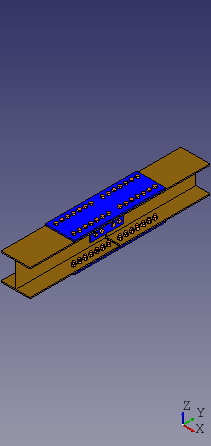
\includegraphics[width=\linewidth]{C:/Users/Priti/Desktop/Osdag3/ResourceFiles/images/3d.png}%
\caption{3D View}%
\end{figure}

%
\end{document}